\documentclass[preprint,authoryear,5p,twocolumn]{elsarticle_mod}

\usepackage{lineno,hyperref}
\usepackage{graphicx} % Required for the inclusion of images
\usepackage{natbib} % Required to change bibliography style to APA
\usepackage{amsmath} % Required for some math elements 
\usepackage{amssymb}
\usepackage{tabularx}
\usepackage{url}
\usepackage{doi}
\usepackage{listings}
\usepackage{mathtools}
\usepackage{multirow}
\usepackage{algorithm}
\usepackage[noend]{algpseudocode}
\renewcommand{\algorithmicensure}{\textbf{Output:}}
\usepackage{etoolbox}
\modulolinenumbers[5]
\lstset{language=Python}
\usepackage{titlesec}

\titlespacing\section{0pt}{12pt plus 4pt minus 2pt}{0pt plus 2pt minus 2pt}
%\usepackage{refcheck}
%%%%%%%%%%%%%%%%%%%%%%%
%% Elsevier bibliography styles
%%%%%%%%%%%%%%%%%%%%%%%
%% To change the style, put a % in front of the second line of the current style and
%% remove the % from the second line of the style you would like to use.
%%%%%%%%%%%%%%%%%%%%%%%

%% Numbered
%\bibliographystyle{model1-num-names}

%% Numbered without titles
%\bibliographystyle{model1a-num-names}

%% Harvard
\bibliographystyle{model2-names.bst}\biboptions{authoryear}

%% Vancouver numbered
%\usepackage{numcompress}\bibliographystyle{model3-num-names}

%% Vancouver name/year
%\usepackage{numcompress}\bibliographystyle{model4-names}\biboptions{authoryear}

%% APA style
%\bibliographystyle{model5-names}\biboptions{authoryear}

%% AMA style
%\usepackage{numcompress}\bibliographystyle{model6-num-names}

%% `Elsevier LaTeX' style
%\bibliographystyle{elsarticle-num}
%%%%%%%%%%%%%%%%%%%%%%%

\begin{document}
%\nocite{*}
\begin{frontmatter}

%\title{Prototype Pulsar Candidate Processing Pipeline for High Volume Data Streams}
\title{SKA Test Vector Pipeline Userguide (v1.1)}
%\tnotetext[mytitlenote]{Fully documented templates are available in the elsarticle package on \href{http://www.ctan.org/tex-archive/macros/latex/contrib/elsarticle}{CTAN}.}

%% Group authors per affiliation:
\author[UOM]{R.~J. Lyon\corref{mycorrespondingauthor}}
\cortext[mycorrespondingauthor]{robert.lyon@manchester.ac.uk (\url{www.scienceguyrob.com})}


%% or include affiliations in footnotes:

\address[UOM]{School of Physics and Astronomy, The University of Manchester, Manchester M13 9PL, UK}

\begin{abstract}
This document describes a software pipeline that generates gold standard test vectors. These are important for validating the performance and correctness of our signal processing tools in radio astronomy. The pipeline is packaged within an easy to use docker container. This allows the pipeline to be on any hardware that can run docker. The primary goal was to make the generation of test vectors reproducible and relatively simple.
\end{abstract}
\end{frontmatter}
\section{Design}
To verify that the prototype software we're building for the SKA correctly meets functional and performance requirements, we require a gold standard set of examples to test with. We refer to the gold standard examples as `test vectors' (TVs). The system used to generate them is referred to as the `test vector generation pipeline' (TVGP).\newline

The TVGP can create example detections of over 1,000 unique pulsar sources, recorded in the EPN database \citep{EPN1:2018,EPN2:2018}. Through attuning TV generation parameters, many more valid permutations of these detections can be created. The pipeline is therefore able to generate an almost infinite number of TVs in practice.\newline

The TVGP is also able to generate `simulated' pulsar examples. These are realistic pulsar examples (i.e. observationally valid) which do not correspond to any known source. Simulated examples fill the pulsar search parameter space not covered by EPN database entries. Using a combination of known and simulated sources, the pipeline is able to generate a variety of examples describing a large proportion of the Galactic pulsar population. This allows the signal recovery capabilities of our code to be probed on common, rare, and unusual sources.\newline

The pipeline has been packaged for distribution inside a Docker image. This is an immutable snapshot of a virtualized software container. It contains all the prerequisites required to execute the TVGP, and the pipeline itself. It is highly recommended that those wishing to use the pipeline obtain the Docker image. Use of the image guarantees that all TVs are generated by a working and identical software environment. Furthermore, by using the ‘dockerised’ pipeline distribution, geographically disjoint teams can generate identical test vectors for cross-group verification. This is the case irrespective of the underlying computing resources used to execute the Docker container. Reproducible test vectors are crucial to ensuring consistency between teams developing and/or testing code.

\section{Sub-elements}
The pipeline consists of a combination of python scripts, pre-existing pulsar search tools, and data collected from the ATNF and EPN pulsar databases. The purpose of each of these pipeline sub-elements is summarized below: 
\begin{enumerate}
\item The Python scripts act as wrappers. These either i) read and manipulate data from ATNF / EPN data sources, or ii) automate the execution of existing pulsar tools to produce test vectors. Primary user interaction with the pipeline is achieved via the Python scripts. The scripts check the validity of user supplied parameters, and simplify pipeline interactions.
\item The pulsar tools perform three crucial tasks. They i) generate noise files which serve as the basis for each test vector, ii) generate pulsar signals which can be inserted into the noise files simulating a genuine telescope observation, and iii) insert the generated pulsar signals into the noise files, to create an observation file ready for processing. Three separate tools are used to undertake these tasks. 
\begin{itemize}
\item \textit{fast\_fake} - generates a single filterbank file containing Gaussian distributed noise more detail on the filterbank file format can be found elsewhere \citep{SIGPROC}. The \textit{fast\_fake} application \citep{FASTFAKE} was created from a fork of the \textit{Sigproc} software suite \citep{SIGPROC}.
\item \textit{Tempo2} - generates a polynomial file that describes the pulse arrival times for a pulsar (i.e. a timing model). Tempo2 is a software suite used primarily for pulsar timing applications \citep{Tempo2,Tempo22}.  
\item \textit{inject\_pulsar} -  takes the model pulse arrival times computed by \textit{Tempo2} for a specific pulsar, and injects the corresponding signal into a filterbank file. The injection process is applied to the noise filterbank file by the pipeline. This produces a new file containing a realistic pulsar signal. Note that the injection process implemented by \textit{inject\_pulsar}, assumes a pulse profile which doesn't change over time. It injects an integrated profile (see Figure \ref{Fig:Profile}), which represents the average pulse recorded over many pulsar rotations (often thousands of rotations). In reality the pulse profile varies greatly with each pulsar rotation, thus this injection method is unrealistic. However, for testing purposes this simplified model is sufficient. It produces realistic test vectors when combined with the noise filterbank file (the noise introduces variation).  The \textit{inject\_pulsar} application was created from a fork of the Sigproc software suite \citep{FASTFAKE}. 
\end{itemize}
\item The ATNF pulsar catalog. This catalog describes all known pulsar sources. The catalog is used to generate parameter files, more generally known as `Par' files. These describe the key characteristics of a pulsar, i.e. pulse period, pulse frequency, dispersion measure, and sky position. Par files are used by the \textit{Tempo2} tool to create a polynomial timing model, which describes pulse arrival times for individual pulsars. 
\item The EPN database describes the integrated pulse profiles of over 1,000 known pulsars. Pulse profiles represent a pulsar detection averaged through both frequency and time. Pulse profiles are useful, as they describe the shape of a pulse, and characterize the principle pulse components. An example profile is shown in Figure 3-2-1. The TVGP uses these integrated profiles to create realistic detections. Profile data is passed to existing pulsar software, and injected into a noise file. Since the EPN database describes the pulse profiles of many pulsars, we can in principle generate examples covering a significant portion of the known pulsar population. 
\end{enumerate}

\begin{figure}
	\centering
		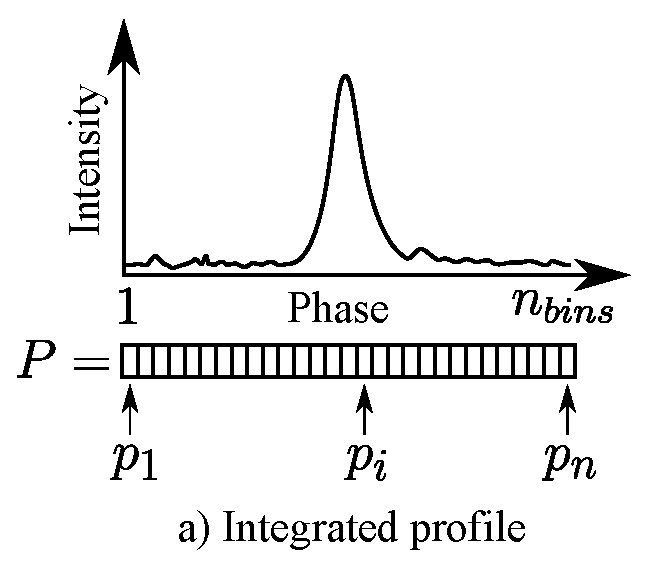
\includegraphics[scale=0.5]{images/eps/Integrated_profile.eps}
		\caption[]{Example of an integrated pulse profile. This describes pulse intensity as a function of phase.}
	\label{Fig:Profile}
\end{figure}

\section{Generation Procedure}
The general test vector generation procedure is as follows: 
\begin{enumerate}
\item 1.	Create a single filterbank file containing only Gaussian distributed white noise. We call this the noise file. This is created using the C software tool \textit{fast\_fake}, using the observational parameters we expect for a standard SKA pulsar search operation. The parameters can be varied according to a user's own requirements.  However for SKA testing, the following parameter values are assumed: 
\begin{itemize}
\item Observation length $T_{obs}$ = 600 seconds. 
\item Sampling interval $T_{samp}$ = 64 microseconds. 
\item Frequency of channel one, $fch1$ = 1350 MHz 
\item Channel bandwidth $\Delta v$ = 78.12500 KHz. 
\item Overall bandwidth $B$ = 320 MHz 
\item Number of channels, $N_{chan}$ = 4096. 
\item Output number of bits = 8. 
\item Random seed for noise generation is 1. 
\end{itemize}
The generated noise file serves as the basis for all test vectors with the same observational parameters.
\item 2.	Before a pulsar signal can be injected into a noise file, some prerequisite files must first be chosen. These include: 
\begin{itemize}
\item A Par file (.par extension) that describes the characteristics of the pulsar whose signal is to be injected. The details are obtained from the ATNF pulsar catalog. 
\item A \textit{Tempo2} predictor file (.dat extension). These can be generated by passing a valid Par file to \textit{Tempo2}. 
\item An ascii file that describes the shape of the pulse to be injected (.asc extension). 
\end{itemize}
These files can be created manually by extracting data from the ANTF catalog (for the .par files), parsing the EPN database (for the .asc files), and by running \textit{Tempo2} with a .par file to create a .dat file. However these files can be found in the TVGP Docker image ready made. Both Par and Tempo2 predictor files have been generated for all pulsars in the ATNF catalog. Whilst .asc files have been created for all entries in the EPN database. Where possible, choose file combinations that correspond to the same pulsar. Where this is not possible (i.e. no EPN data available), either choose an appropriate substitute file, or create one manually (i.e. create a .asc file). Note: choosing files which do not correspond to the same pulsar, will create a new simulated pulsar test vector (as opposed to a known source example).
\item To inject a pulsar signal, the \textit{inject\_pulsar} tool is used. It requires i) a noise file, ii) a .dat file, and iii) a .asc file. When running \textit{inject\_pulsar} the random seed is always set to 1. This is done to ensure that test vectors are reproducible. All other injection parameters are assigned their default values. Once the \textit{inject\_pulsar} command has been executed, a new filterbank file is produced. This is the test vector ready for further analysis. 
\end{enumerate}

\section{Architecture}
The pipeline architecture is relatively simple. An overview is presented in Figure \ref{Fig:Arch}. Here we see the pipeline hosted within a Docker container, running upon an arbitrary host OS. The container itself runs a minimal CentOS 7 environment. This environment includes a variety of software packages, required to run the pulsar tools that perform the test vector generation. User interaction with the pipeline is generally achieved via a collection of Python scripts. These interact with the pulsar tools and a variety of .dat and .asc files, to generate TVs. Note that the .dat and .asc files are used as inputs to the pulsar tools. These files are usually created manually. However the pipeline Docker image comes with these files pre-made. There are four data directories containing pre-made data worthy of note:\newline

\textbf{ASC} - This directory contains files which describe pulse profiles extracted from the EPN database. Each file in the directory is named as follows:\newline 

$<$Pulsar name$>$\_$<$Frequency$>$.asc \newline 

Where $<$Pulsar name$>$ is the pulsar 'J' name, and $<$Frequency$>$ the observation frequency of the EPN data. There is a single file per each unique entry in the EPN database, representing observations covering a wide range of frequencies. The files themselves are stored in comma separated value (CSV) format. They contain the total pulse intensity observed (the I stokes parameter) written to a single line of ascii text. For example:\newline
 
0,1,2,3,11,29,67,180,71,39,9,2,1,1,1,0 \newline

has 16 bins, each describing total pulse intensity. Note that the intensity values stored in the files are scaled to a $[0,255]$ range. This directory also contains a python script \textit{EpnToAsc.py}. This converts files from the EPN database to .asc files. In total there are 3,698 .asc files available (~30 MB of data).\newline
 
\textbf{EPN\_Raw} -  This directory contains 3,698 files extracted from the EPN database. These describe pulsar profiles in plain text files. The files are named as follows:\newline

$<$Pulsar name$>$\_$<$Freq.$>$.acn \newline

or 

$<$Pulsar name$>$\_$<$Freq.$>$\_$<$Number$>$.acn \newline

if there is more than one EPN file representing a pulsar observed at the specified frequency. These files are space delimited. More details about the files can be found online at \url{http://www.epta.eu.org/epndb/}.\newline

The data in this directory were obtained from the EPN database under the Creative Commons Attribution 4.0 International license. We gratefully acknowledge the authors of the EPN database (past and present), and those who have contributed data to it over the years.  Data was extracted from the EPN database on March 15th 2016. In total there are 3698 files available (~65 MB of data).\newline
 
\textbf{PARS} - This directory contains Par files for real pulsars. These Par files were generated by the \textit{CandidateParGenerator.py} script. To create these files, the script reads a valid ATNF pulsar catalog database file. It extracts the RA, DEC, period, and DM values per source, and stores these in a valid par file. The Par files were generated using pulsar catalog version 1.54. In total there are 2,536 par files available (~11 MB of data).\newline
 
\textbf{PREDS} - This directory contains \textit{Tempo2} predictor (.dat) files. The files it contains correspond to real pulsars. These files were generated by \textit{Tempo2} version 2014.11.1, using the Par files in the PARS folder. In total there are 2,536 predictor files available (~425 MB of data).\newline

Once the pulsar tools have generated a new TV file, it is persisted to a host disk drive. This ensures the TV persists after the software container has been discarded. 

\begin{figure*}
	\centering
		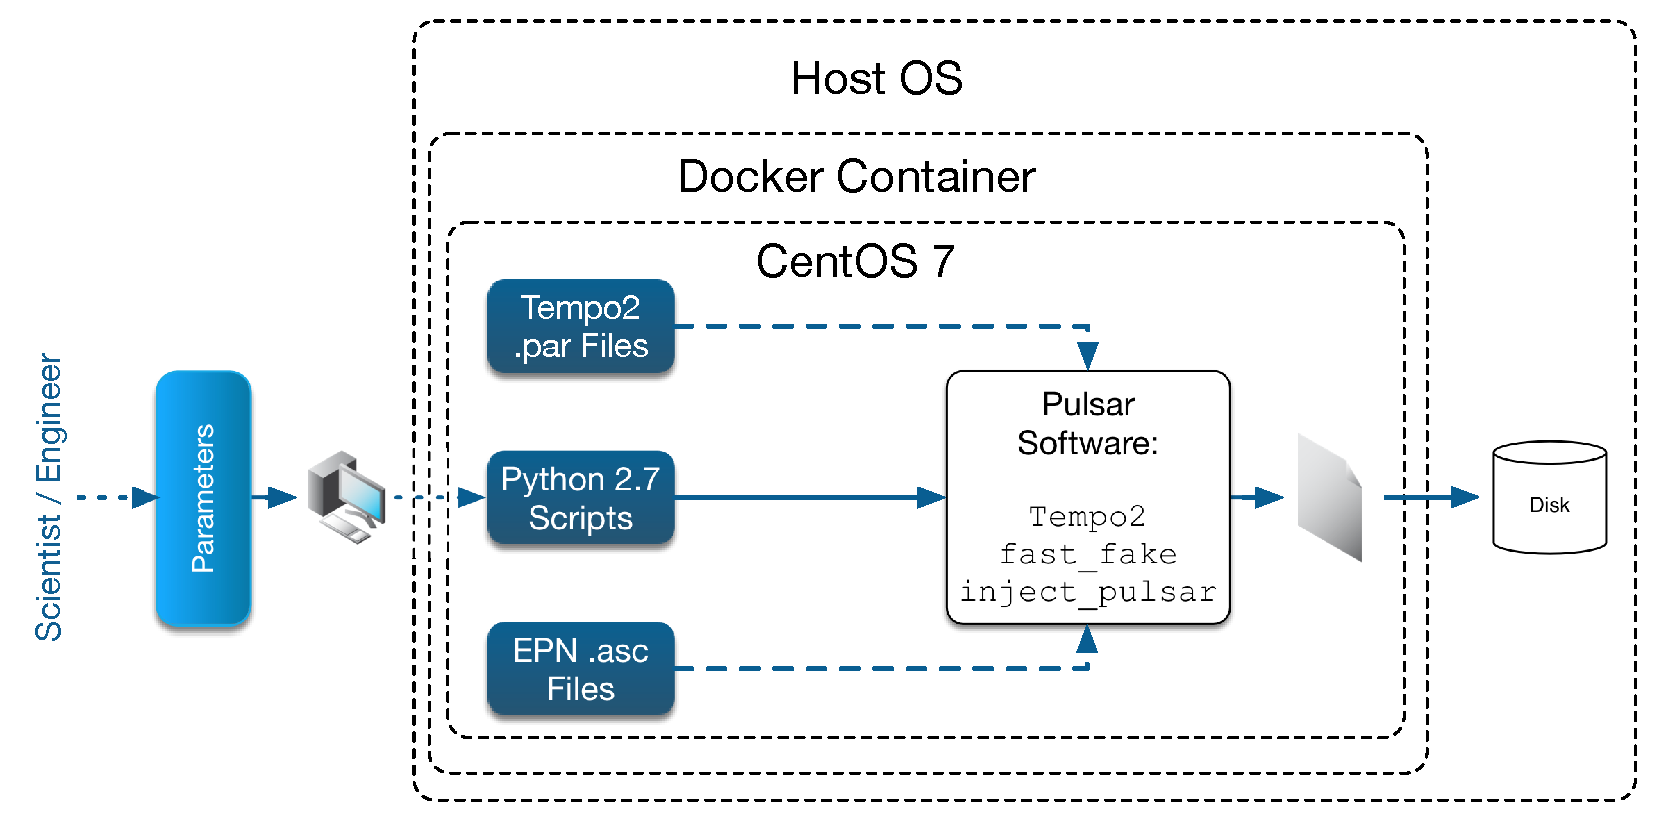
\includegraphics[scale=0.5]{images/eps/TestVectorDiagrams.eps}
		\caption[]{Test vector generation pipeline architecture.}
	\label{Fig:Arch}
\end{figure*}

\section{Noise File Generation}
The first step in test vector generation involves creating a noise file. This is a one time only step. The noise file forms the basis of all subsequent test vectors. The noise file creation process is summarized in Figure A-6-1. This process is extremely simple. The user simply executes the \textit{fast\_fake} tool using their desired observation parameters. During this step RFI may also be inserted into the noise file using pulsar software in the Docker container. 
\begin{figure}
	\centering
		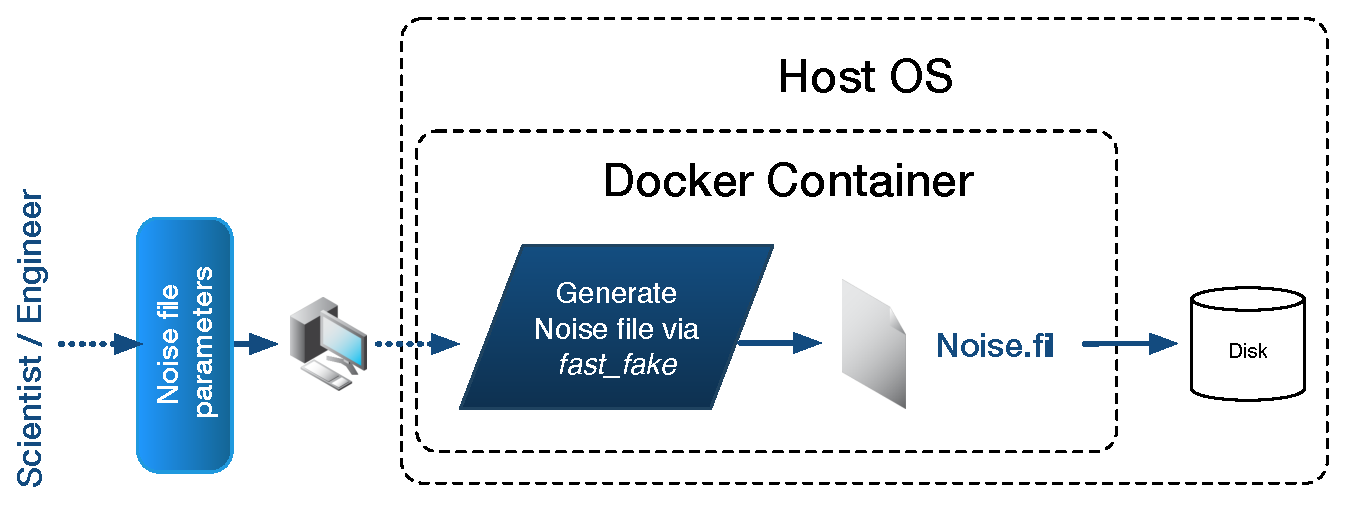
\includegraphics[scale=0.4]{images/eps/NoiseGen.eps}
		\caption[]{Noise file generation.}
	\label{Fig:Noise}
\end{figure}
\section{Prerequisite Generation}
The prerequisite steps have already been undertaken for the TVGP. However the user may wish to regenerate these files, or generate new files to simulate more pulsars. The prerequisite generation steps are summarized in Figure \ref{Prereq}. The general steps are: 
\begin{enumerate}
\item Create a Par file describing a pulsar or simulated pulsar source. Par files can either be generated manually, or using the \textit{CandidateParGenerator.py} script bundled with the TVGP. 
\item Create a predictor file for the new Par file using \textit{Tempo2}. The Par file created in step 1 is given to \textit{Tempo2}, and a new .dat predictor file is created. \textit{Tempo2} can either be run manually, or via the script \textit{GeneratePredictorFiles.py}. 
\item Choose a .asc file describing a pulse profile. This file is used to describe the shape of the pulsar signal to be inserted into the test vector. The .asc files can be chosen manually. However it is better to use the \textit{InjectPulsarCommandCreator.py} script to automatically choose the .asc files.
\end{enumerate}
\begin{figure}
	\centering
		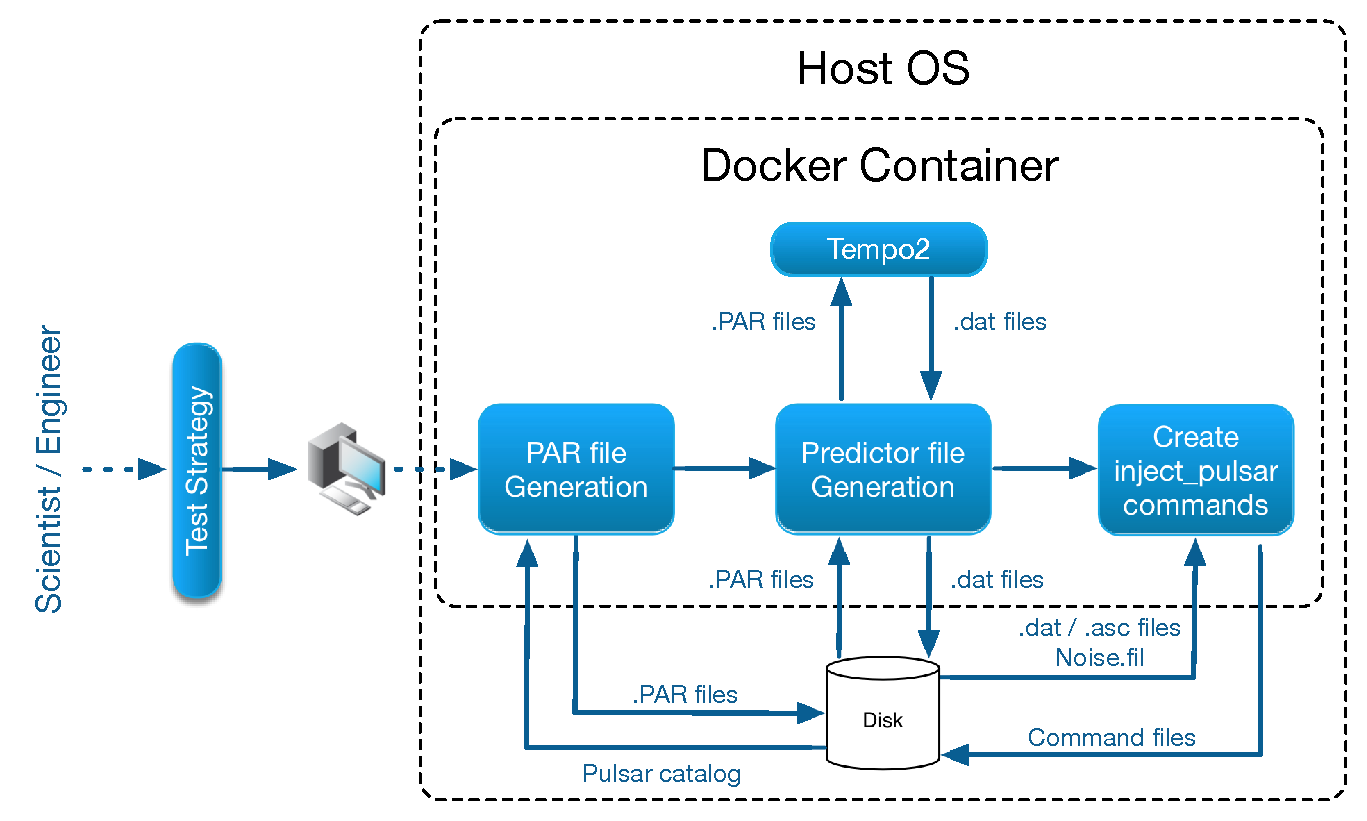
\includegraphics[scale=0.4]{images/eps/DataFlow.eps}
		\caption[]{Overview of test vector prerequisite file generation.}
	\label{Fig:Prereq}
\end{figure}

\section{Signal Injection}
Once all the prerequisite files are available, pulsar signals can be injected into a new copy of the previously generated noise file. This involves running the \textit{inject\_pulsar} tool. The tool can be run manually, however it is recommended that the user run the \textit{InjectPulsarAutomator.py} script instead. This script simply executes shell commands which invoke \textit{inject\_pulsar} using the correct input parameters. The shell commands are generated using the \textit{InjectPulsarCommandCreator.py} script. 
\begin{figure*}
	\centering
		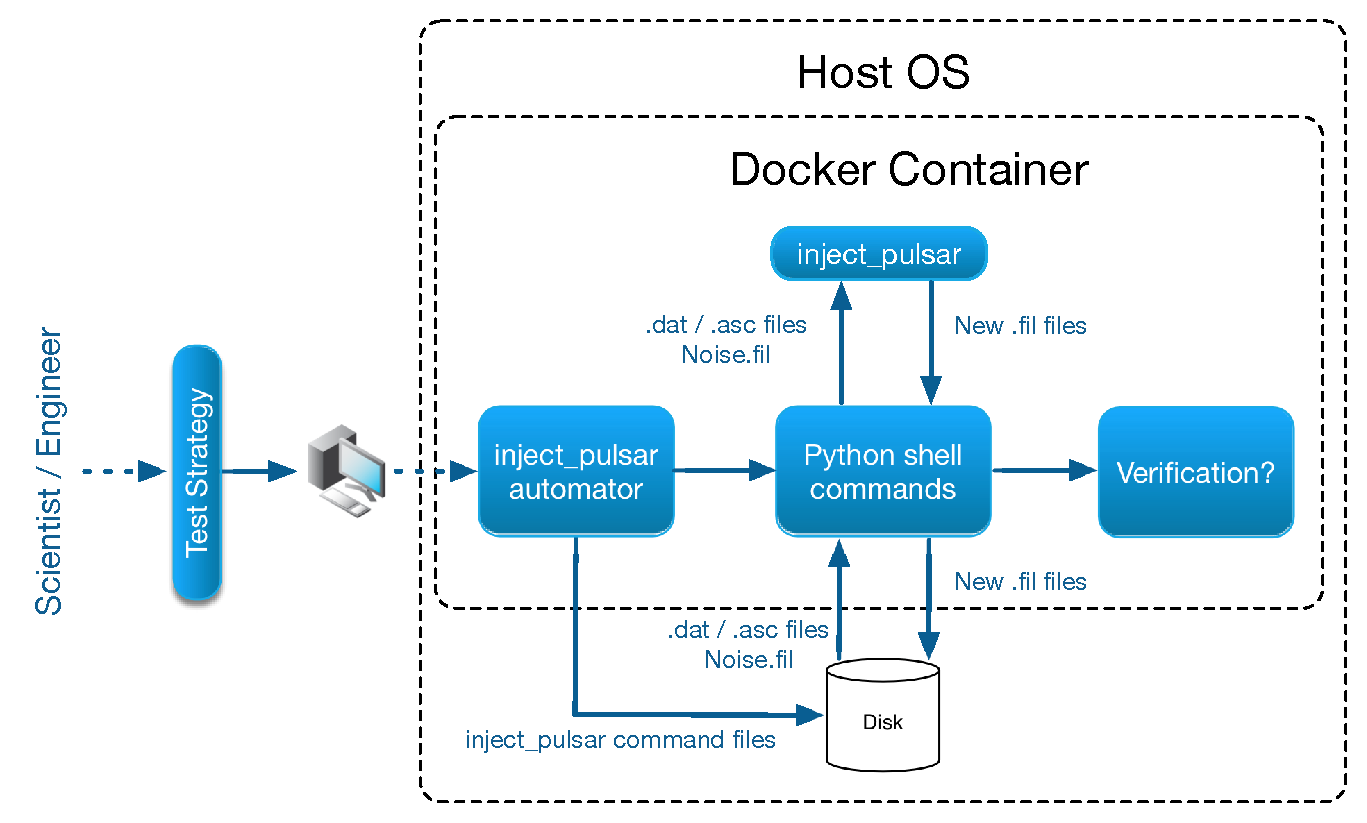
\includegraphics[scale=0.5]{images/eps/Prereqs.eps}
		\caption[]{Overview of how pulsar signals are injected into noise files. }
	\label{Fig:Injection}
\end{figure*}

\section{Provided Software}
Scripts have been written to automate the creation of test vectors. These include: 
\begin{itemize}
\item \textit{CandidateParGenerator.py} - this script generates Par files for ATNF catalog sources, and Par files, for fake pulsars created via sampling user specified distributions over pulse period, S/N, and DM. The script is compatible with python version 2.7. It requires Scipy version 0.15 or later to function. Numpy 1.0 or later, and Matplotlib version 1.5 or later are also required.
\item \textit{GeneratePredictorFiles.py} - this automatically generates Tempo2 (Tempo2 version 2014.11.1) predictor files for any Par files found in a user supplied directory. The script is compatible with python version 2.7.  It requires Tempo2 version 2014.11.1, Scipy version 0.15 or later to function. Numpy 1.0 or later, and Matplotlib version 1.5 or later are also required.
\item \textit{InjectPulsarCommandCreator.py} - this generates a file containing \textit{inject\_pulsar} commands, useful for batching the creation of filterbank files containing pulsar signals. The script locates the correct .asc files for legitimate pulsars when creating the \textit{inject\_pulsar} commands. For fake pulsar Par files (generated by \textit{CandidateParGenerator.py}), the script will randomly choose an available .asc file, thereby creating a fake pulsar example using realistic profile data. It is possible to audit which .asc files were allocated to fake pulsars. The script is compatible with python version 2.7.  It requires Scipy version 0.15 or later to function. Numpy 1.0 or later, and Matplotlib version 1.5 or later are also required. 
\item \textit{InjectPulsarAutomator.py} - this script reads the files output by \textit{InjectPulsarCommandCreator.py} (version 1.0), and executes the commands. The script is compatible with python version 2.7.  It requires Scipy version 0.15 or later to function. Numpy 1.0 or later, and Matplotlib version 1.5 or later are also required. 
\end{itemize}
The software can be found in the home folder of the Docker image. 

\section{Use}
To execute Docker commands you have to use the \textit{sudo} command. Below are examples of the main Docker commands available.\newline
 
sudo docker login \newline

The login command logs a user into the Docker hub. An account is required if a user wants to download the latest test vector pipeline image, or upload their own Docker images.\newline
 
sudo docker images\newline
 
This command prints out details of the Docker images available on the local machine. These are the images available to run locally.\newline
 
sudo docker build -t $<$docker file$>$.
 
This command builds a new Docker software container, based on the user specified Docker file. Note the full stop at the end of the command - this is required and isn’t a typo.\newline

sudo docker push $<$docker file$>$\newline

This command uploads the software container built using the specified Docker file, to the Docker hub (needs an account and valid user login credentials).\newline

sudo docker rmi -f $<$image id$>$\newline
 
This command deletes a local Docker image from the host machine. Useful if an image is faulty, or if disk space is low. To find the Docker image ID’s, run the sudo docker images command.\newline
 
sudo docker pull $<$docker file$>$\newline
 
This command pulls a Docker image from the Docker hub.\newline
 
sudo docker run -it -v $<$local dir path$>$:$<$docker image dir path$>$ $<$docker file$>$\newline
 
This command runs a Docker image locally. The -v flag tells the Docker engine to mount a host file directory, inside the Docker container. This allows files to be copied between the host, and a Docker container. The flags used above:\newline
\begin{itemize}
\item -i is the interactive flag
\item -t tells Docker to open a terminal 
\item -v mounts a volume
\end{itemize} 

The ordering of flags and parameters matters. Put all the flags and parameters before the Docker image is specified. 

\textbf{Caveats:} \newline
When using the -v flag: if a $<$path to create in image$>$ is supplied that already exists in the Docker image, then any files there will be overwritten, if they exist in $<$path to local folder$>$. 

\subsection{Example Usage} 
\noindent\begin{minipage}{.95\textwidth}
Here we list the available images: 
\begin{lstlisting}[language=bash]
[lyon@zeus ~]$ sudo docker images 
[sudo] password for lyon:  
REPOSITORY              TAG      IMAGE ID           CREATED           SIZE 
my-docker-image        latest   19e0164251da        8 days ago       84.91MB 
debian                 wheezy   34a0b91d4fe9        13 days ago      84.91 MB 
scienceguyrob/ska-test-vectors   latest   44ddec452b70        2 weeks ago      3.521 GB 
hello-world            latest   c54a2cc56cbb        4 months ago     1.848 kB 
\end{lstlisting}

Here we run a Docker image: 

\begin{lstlisting}[language=bash]
[lyon@zeus ~]$ sudo docker run -it scienceguyrob/ska-test-vectors 
root@3c6064b40e3b:~# ls 
DockerImageReadme.txt  psr 
root@3c6064b40e3b:~#
\end{lstlisting}

Here the directory loaded upon login is home. It contains a single text file and the folder psr. To create a test vector, we first generate a 10 second noise file. Note the following commands require some knowledge of pulsars, and pulsar searching. Such knowledge helps understand the parameters chosen, and the tools used to study the data. It is not within the scope of this document to provide such knowledge.
\begin{lstlisting}[language=bash]
root@3c6064b40e3b:~# fast_fake --tobs 1 --tsamp 64 --fch1 1350 --foff -0.078125
 --nbits 8 --nchans 4096 --seed 1 > noise.fil 
[fast_fake.c:101] FASTFAKE - M.Keith 2014 
[fast_fake.c:110] tobs          = 1.000000s 
[fast_fake.c:111] tsamp         = 64.000000us 
[fast_fake.c:112] mjdstart      = 56000.000000 
[fast_fake.c:113] freq chan 1   = 1350.000000MHz 
[fast_fake.c:114] freq offset   = -0.078125MHz 
[fast_fake.c:115] output nbits  = 8 
[fast_fake.c:116] random seed   = 1 
[fast_fake.c:117] output file   = 'stdout' 
[fast_fake.c:128] write header 
[fast_fake.c:160] Generate 15625 samples, 0.060 GiB 
Complete:  100%. Sample:     15600 Real time    4.0s, Sim time    1.0s. Speed  15.23MiB/ss 
[fast_fake.c:246] Done! 
root@3c6064b40e3b:~#
\end{lstlisting}
\end{minipage}\clearpage

\noindent\begin{minipage}{.95\textwidth}
Next we insert a pulsar signal. We choose J0332+5434 (B0329+54) as our example pulsar. The signal inserted is based on data taken from the EPN database. This data describes an observation of the pulsar at 1400 MHz.

\begin{lstlisting}[language=bash]
root@3c6064b40e3b:~# inject_pulsar --snr 15 --seed 1 --pred /home/psr/soft/
pulsar_injection_pipeline/PREDS/J0332+5434.dat --prof /home/psr/soft/
pulsar_injection_pipeline/ASC/J0332+5434_1400.asc noise.fil > J0332+5434_1400.fil 
[inject_pulsar.c:164] Disable scattering/scintillation 
[inject_pulsar.c:177] input .fil file = 'noise.fil' 
[inject_pulsar.c:178] Predicor     = '/home/psr/soft/pulsar_injection_pipeline/
PREDS/J0332+5434.dat' 
[inject_pulsar.c:179] Profile      = '/home/psr/soft/pulsar_injection_pipeline/
ASC/J0332+5434_1400.asc' 
[inject_pulsar.c:185] Target S/N   = 15.00 
[inject_pulsar.c:186] Ref Freq     = 1400.00 MHz 
[inject_pulsar.c:187] Spectrum     = f^(-1.50) 
[inject_pulsar.c:188] t_scatter    = (0 s) * f^(-4.00) 
[inject_pulsar.c:189] scint_bw     = 0 MHz 
[inject_pulsar.c:190] Random Seed  = 0x1 
[inject_pulsar.c:224] Input Nsamples  = 15625 
[inject_pulsar.c:225] Input Tobs      = 1.000000 
[inject_pulsar.c:226] Input Nchans    = 4096 
[inject_pulsar.c:248] Initialising convolution plans. 
[inject_pulsar.c:253] read profile file 
[inject_pulsar.c:326] best_sum=693.42 scale=6.48957e-05, width=1 
[inject_pulsar.c:370] Pulsar period ~714.52ms 
[inject_pulsar.c:421] Tscatter@1400.0MHz = 0s 
[inject_pulsar.c:422] Tscatter@1350.0MHz = 0s 
[inject_pulsar.c:423] Tscatter@1030.1MHz = 0s 
[inject_pulsar.c:483] Generated 1 ISM models 
[inject_pulsar.c:490] Starting simulation 
15360 samples,  1.0s 
[inject_pulsar.c:598] Simulation ended. 
[inject_pulsar.c:599] last sample=56000.00001157407407 
[inject_pulsar.c:600] Setup took   0.11 s 
[inject_pulsar.c:601] Process took 2.02 s 
[inject_pulsar.c:602] >> Inner took  0.50 s 
[inject_pulsar.c:603] >> Read took  0.37 s 
[inject_pulsar.c:604] >> Write took  0.28 s 
[inject_pulsar.c:605] Total was  2.1 times 'real' time 
[inject_pulsar.c:606] Check last Random 329f47ba 
root@3c6064b40e3b:~# 
root@3c6064b40e3b:~# ls 
DockerImageReadme.txt  J0332+5434_1400.fil  noise.fil  psr 
root@3c6064b40e3b:~#
\end{lstlisting}
As can be seen above, a new filterbank file has been created called J0332+5434\_1400.fil. This describes an observation of the pulsar J0332+5434. The following steps de-disperse the data, and create a file describing the pulse profile. 
\begin{lstlisting}[language=bash]
root@3c6064b40e3b:~# dedisperse J0332+5434_1400.fil -d 26.7641 -o J0332+5434_1400.tim 
root@3c6064b40e3b:~# /home/psr/soft/sigproc/install/bin/fold J0332+5434_1400.tim -p
0.71451969972 -o J0332+5434_1400.prf 
root@3c6064b40e3b:~# ls 
DockerImageReadme.txt  J0332+5434_1400.fil  noise.fil  J0332+5434_1400.prf  J0332+5434_1400.tim  psr 
root@3c6064b40e3b:~#  
\end{lstlisting}\end{minipage}\clearpage

If the data stored in the file J0332+5434\_1400.prf is repeated, and then plotted, we obtain the following integrated pulse profile. 
\begin{figure}
	\centering
		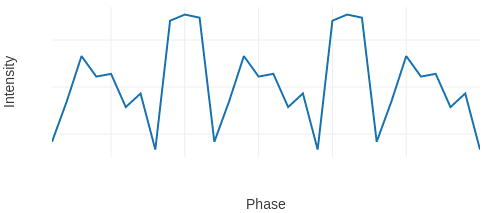
\includegraphics[scale=0.4]{images/png/SimulatedPulse.png}
		\caption[]{Noise file generation.}
	\label{Fig:Noise}
\end{figure}

\begin{thebibliography}{1}
\bibitem[\protect\citeauthoryear{Lorimer et. al.}{1997}]{EPN1:2018}
{Lorimer} D.R. et. al., 1997, ``The European Pulsar Network Pulse Profile Database", Joint European and National Astronomical Meeting, JENAM-97. 6th European and 3rd Hellenic Astronomical Conference, Thessaloniki, Greece, 2-5 July, 1997.

\bibitem[\protect\citeauthoryear{Keith}{2018}]{EPN2:2018}
{Keith} M.~J., 2018, ``The EPN database of pulsar profiles", on-line, \url{http://www.epta.eu.org/epndb/}, accessed 26/04/2018.

\bibitem[\protect\citeauthoryear{Lorimer}{2018}]{SIGPROC}
{Lorimer} D.R., 2018, ``SIGPROC: Pulsar Signal Processing Programs", on-line, \url{http://sigproc.sourceforge.net}, accessed 26/04/2018.

\bibitem[\protect\citeauthoryear{Keith}{2018}]{FASTFAKE}
{Keith} M.~J., 2018, ``SixByNine/sigproc", on-line, \url{https://github.com/SixByNine/sigproc}, accessed 26/04/2018.

\bibitem[\protect\citeauthoryear{Hobbs et. al.}{2006}]{Tempo2}
{Hobbs} G. et. al., 2006, ``Tempo2: a New Pulsar Timing Package", Chinese Journal of Astronomy and Astrophysics, vol. 6, S2, 2006. 

\bibitem[\protect\citeauthoryear{Hobbs et. al.}{2018}]{Tempo22}
{Hobbs} G. et. al., 2018, ``Tempo2", on-line, \url{http://www.atnf.csiro.au/research/pulsar/tempo2/}, accessed 26/04/2018. 

\end{thebibliography}

\end{document}

